\section{Experiment}

\subsection{The purpose of experiment}
There are some questions that we care about.Soving these problems through controlled experiment we prove that TGCT are meaningful.RQ1: Is the tool-based crowdsourcing testing effective in improving the efficiency of crowdsourcing testing? RQ2: Does static analysis effectively guide the crowd workers to improve the coverage of crowdsourcing testing? 

\subsection{The setup of experiment}
The experiment selected three Android apps: "Jiandou", "QQ Video" and "Music Club".Each application sets up three sets of control experiments during the test: traditional crowdsourcing testing, crowdsourcing testing that only includes automated test guidance, and crowdsourcing testing guided by automated testing and static analysis(TGCT).we define |C| as the traditional crowdsourcing testing process, |A| as only partially guided crowdsourcing testing,|T| as the TGCT mechanism.

\subsection{The result of experiment}
In order to answer RQ1, we define the efficiency of the crowdsourcing test as the number of exceptions triggered per unit time. In the experiment |C| and |T|, the number of non-repeating exceptions that the crowd workers discovered had been counted every minute. We got three line charts of the number of exceptions in three applications over time, as shown in Figure\ref{fig:xi}.
\begin{figure}[htbp]
\centering
\centerline{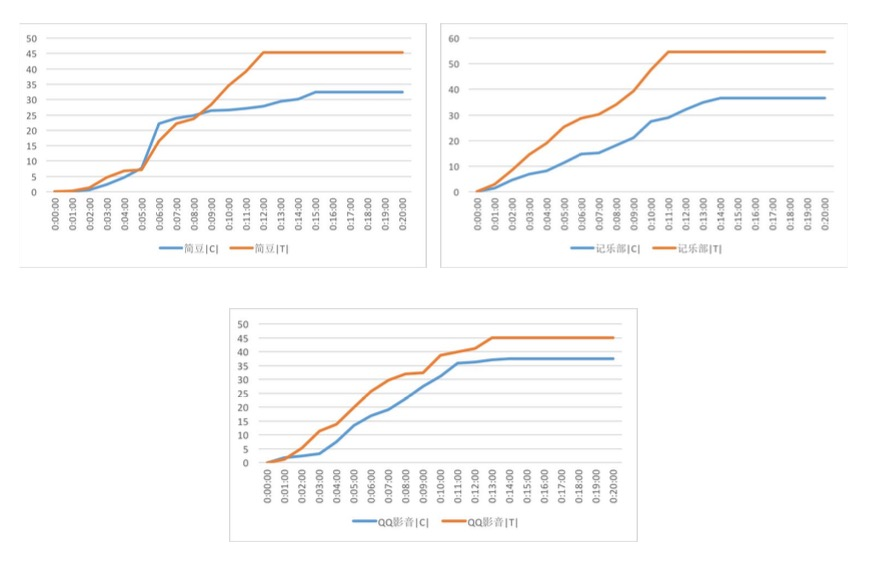
\includegraphics[width=\columnwidth,height=5cm]{fig/8.png}}
\caption{Line chart of the number of exceptions in three applications over time.}
\label{fig:xi}
\end{figure}
From the overall trend of the three figures, tool-led crowd workers trigger exceptions faster and more.

In order to answer RQ2, we count the proportion of windows that are not covered by these three applications, as shown in Figure\ref{fig:xixi}.
\begin{figure}[htbp]
\centering
\centerline{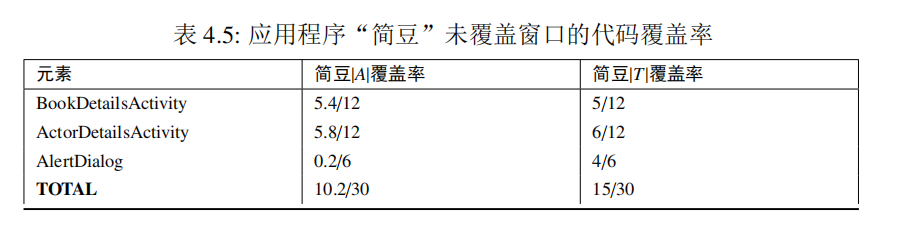
\includegraphics[width=\columnwidth,height=10cm]{fig/9.png}}
\caption{coverage statistics}
\label{fig:xixi}
\end{figure}

Then we compare the result of experiment |T| with the experiment |A| to verify the effectiveness of the boot mechanism for uncovered window jumps according to the average code coverage of the starting window.
According to the calculation results of all the code coverage of the uncovered window, we found that for crowd workers, the guidance of static source analysis can effectively improve the coverage of crowdsourcing testing.